\providecommand{\zkTBC}[1]{\textbf{[TO COMPLETE: #1]}}

\section{Characterizing zkML Serving Workloads}
\label{sec:characterization}

We characterize the properties of partitioned zkML workloads that shape
scheduling in a shared prover. We focus on three questions: how partitioning
changes proving cost, how runtime and memory vary across proof jobs, and how
memory demand evolves within a job.

\subsection{Workloads and Measurement Method}
\label{sec:characterization-method}

We use TinyBERT, MobileNetV2, and NanoGPT (4L), spanning convolutional,
encoder, and autoregressive models. At the finest granularity they produce
120, 100, and 181 proof jobs, respectively. We compare monolithic proving
with partitioned proving in which all jobs execute sequentially on the same
prover, isolating the effect of proving granularity from inter-job parallelism.
Both use EZKL~\cite{ezkl} on a dual-socket AMD EPYC 9354 server with
755~GiB of RAM. We record per-job execution time, process memory, and major
proof-stage transitions. Unless otherwise stated, runs begin cold so that the
full setup and proving lifecycle is represented.

\subsection{Impact of Partitioning on Proving Cost}
\label{sec:decomposition-benefit}

Figure~\ref{fig:partition-benefits} shows that partitioning reduces proving
time even when jobs execute serially. Relative to monolithic proving,
completion time falls by 40.6\% for TinyBERT, 16.3\% for MobileNetV2, and
60.5\% for NanoGPT (4L). Peak memory falls by 80.5\%, 91.5\%, and 98.0\%,
respectively. Partitioning also makes larger models feasible: monolithic
NanoGPT (10L) exhausts available memory, whereas partitioned execution
completes with a 12.0~GiB peak.

\textbf{Implication.}
Partitioning changes the workload presented to the runtime by reducing the
cost and memory footprint of individual proof jobs while exposing additional
parallelism.

\begin{figure}[t]
    \centering
    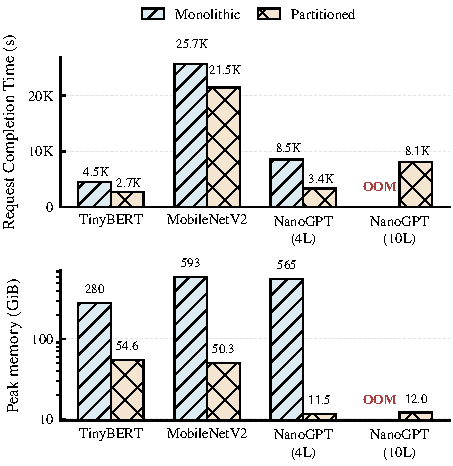
\includegraphics[width=\columnwidth]{figures/sacdad/partitioning_benefits.pdf}
    \caption{Monolithic and partitioned proving. Partitioned request time is
    the sum of proof-job runtimes; memory is the largest observed job footprint.
    OOM indicates that proving exceeded available memory.}
    \label{fig:partition-benefits}
\end{figure}

\begin{figure*}[t]
    \centering
    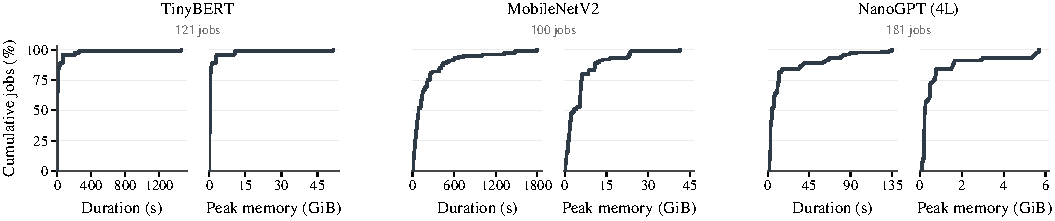
\includegraphics[width=\textwidth]{figures/sacdad/job_heterogeneity.pdf}
    \caption{Empirical distributions of proof-job execution time and peak
    memory for TinyBERT, MobileNetV2, and NanoGPT (4L).}
    \label{fig:job-heterogeneity}
\end{figure*}

\subsection{Heterogeneity Across Proof Jobs}
\label{sec:job-heterogeneity}

Figure~\ref{fig:job-heterogeneity} shows substantial heterogeneity within
each request. TinyBERT's longest job takes 1,461.3~s compared with a 4.47~s
median, a \(327\times\) difference, and accounts for 40.9\% of aggregate
job time. MobileNetV2 and NanoGPT show smaller but still substantial spreads
of approximately \(21\times\) and \(31\times\).

Memory is similarly uneven. Median per-job peaks are 0.21, 3.38, and
0.22~GiB for TinyBERT, MobileNetV2, and NanoGPT, while the largest reach
51.61, 41.45, and 5.70~GiB. A fixed concurrency limit therefore says little
about either remaining request work or instantaneous memory pressure.

\textbf{Implication.}
Runtime estimates help identify jobs that may dominate request completion,
while memory estimates determine which jobs can safely share a prover node.

\begin{figure*}[t]
    \centering
    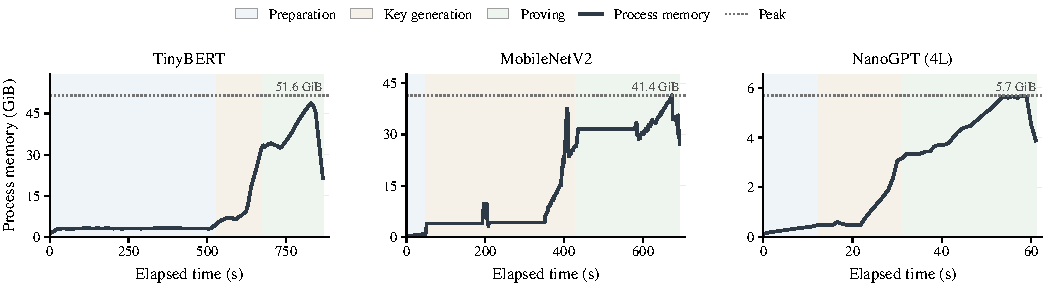
\includegraphics[width=\textwidth]{figures/sacdad/stage_memory.pdf}
    \caption{Memory demand over time for the highest-memory proof job in each
    workload. Shaded regions identify preparation, key generation, and proving.}
    \label{fig:stage-memory}
\end{figure*}

\begin{table}[t]
\centering
\setlength{\tabcolsep}{5pt}
\renewcommand{\arraystretch}{1.1}
\begin{tabular}{lcc}
\toprule
Workload & \shortstack{Time at $\geq90\%$\\of peak (\%)} &
\shortstack{Peak / average\\memory} \\
\midrule
TinyBERT      & 4.8  & $4.07\times$ \\
MobileNetV2   & 3.5  & $2.53\times$ \\
NanoGPT (4L)  & 13.3 & $2.22\times$ \\
\bottomrule
\end{tabular}
\caption{Temporal variation in memory demand for the highest-memory job in
 each workload.}
\label{tab:temporal-memory}
\end{table}

\subsection{Resource Demand Across Execution Stages}
\label{sec:stage-resource-demand}

Peak memory does not reveal how demand evolves during execution. We therefore
align process-memory samples with preparation, key generation, and proving.
Figure~\ref{fig:stage-memory} shows that the highest-memory jobs spend only
4.8\%, 3.5\%, and 13.3\% of execution at or above 90\% of peak memory for
TinyBERT, MobileNetV2, and NanoGPT, respectively. Their peaks are
\(4.07\times\), \(2.53\times\), and \(2.22\times\) their time-averaged
memory consumption (Table~\ref{tab:temporal-memory}).

\textbf{Implication.}
Whole-job peak reservation is conservative for much of execution. A runtime
can expose additional concurrency by admitting stages according to their
current memory demand rather than reserving every job's eventual peak for its
entire lifetime.

\begin{figure*}[t]
    \centering
    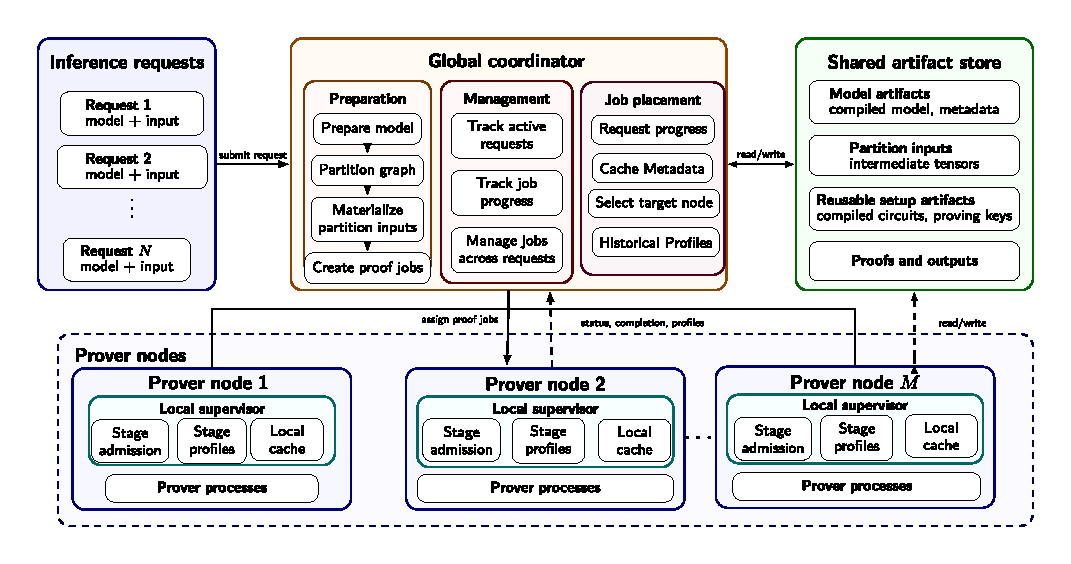
\includegraphics[width=\textwidth]{figures/sacdad/architecture.pdf}
    \caption{Architecture of \TITLE{}. A global coordinator places proof jobs
    across prover nodes, while each node performs local stage admission using
    current memory availability and historical resource profiles.}
    \label{fig:architecture}
\end{figure*}
